\subsection{Distribution of the Determinant of a Complex-Valued Sample Correlation Matrix}

\emph{In this post, we look at the distribution of the determinant of the sample correlation matrix of the realizations of a complex-valued Gaussian random vector. The distribution for real-valued Gaussian random vector was developed in \cite{PhamGia2014}, and we largely follow the developed framework. Thanks to Prashant Karunakaran for bringing this problem and the many applications to my attention in late 2017/early 2018.}

Let $\boldsymbol{x}$ be a Gaussian random vector of length $p$ with mean $\boldsymbol{\mu} \in \mathbb{C}^p$ and covariance $\boldsymbol{\Sigma} \in \mathbb{C}^{p\times p}.$ Let $\boldsymbol{x}^{(1)}, \boldsymbol{x}^{(2)}, \dots, \boldsymbol{x}^{(n)}$ denote $n$ realizations, $n \geq p,$ of $\boldsymbol{x}.$ In the terminology of \cite{PhamGia2014}, the adjusted sample covariance matrix is given by $$\boldsymbol{S} = \frac{1}{n}\sum_{i = 1}^{n}(\boldsymbol{x}^{(i)} - \bar{\boldsymbol{x}})(\boldsymbol{x}^{(i)} - \bar{\boldsymbol{x}})^\mathrm{H},$$ where $\bar{\boldsymbol{x}}$ is the sample mean given by $$\bar{\boldsymbol{x}} = \frac{1}{n}\sum_{i = 1}^{n}\boldsymbol{x}^{(i)}.$$ Note that the adjusted sample covariance matrix is positive semi-definite.

The correlation matrix $\boldsymbol{R}$ is defined as: $$\boldsymbol{R} = \boldsymbol{D}^{-\frac{1}{2}} \boldsymbol{S} \boldsymbol{D}^{-\frac{1}{2}},$$ where $\boldsymbol{D} = \mathrm{Diag}(\boldsymbol{S})$ is a diagonal matrix with the diagonal elements of $\boldsymbol{S}$ on the main diagonal. Hence, $\boldsymbol{R}$ has unit diagonal elements and is independent of the variance of the elements of $\boldsymbol{x}.$ 

Now, for real-valued $\boldsymbol{x},$ the determinant of $\boldsymbol{R},$ denoted by $|\boldsymbol{R}|,$ is shown in \cite[Theorem 2]{PhamGia2014} to be a product of $p-1$ Beta-distributed scalar variables $\mathrm{Beta}(\frac{n-i}{2},\frac{i-1}{2}),$  $i=1,\dots,p-1.$ The density of the product can be given in terms of the \href{https://mathworld.wolfram.com/MeijerG-Function.html}{$\mathrm{MeijerG}$ function} as follows \cite[Theorem 2]{PhamGia2014}:

$$g_\mathbb{R}(x;n,p) = \frac{\left[\Gamma(\frac{n-1}{2})\right]^{(p-1)} }{\Gamma(\frac{n-2}{2})\dots\Gamma(\frac{n-p}{2})} \mathrm{MeijerG}^{\begin{bmatrix}p-1 & 0 \\ p-1 & p-1\end{bmatrix}}\left(x\middle|\begin{matrix}\frac{n-3}{2},\dots,\frac{n-3}{2}\\ \frac{n-4}{2},\dots,\frac{n-(p+2)}{2}\end{matrix}\right).$$

Analogously, for complex-valued $\boldsymbol{x},$ $|\boldsymbol{R}|$ is a product of $p-1$ Beta-distributed scalar variables $\mathrm{Beta}(n-i,i),$  $i=1,\dots,p-1.$ The density of the product can now be given in terms of the $\mathrm{MeijerG}$ function, in a straightforward manner, as follows.

$$g_\mathbb{C}(x;n,p) = \frac{\left[\Gamma(n-1)\right]^{(p-1)} }{\Gamma(n-1)\dots\Gamma(n-p+1)} \mathrm{MeijerG}^{\begin{bmatrix}p-1 & 0 \\ p-1 & p-1\end{bmatrix}}\left(x\middle|\begin{matrix}n-1,\dots,n-1\\ n-2,\dots,n-p\end{matrix}\right).$$

In the following, a Mathematica program for numerical simulation and the corresponding output are provided.

\begin{lstlisting}[language=Mathematica,numbers=none]
gC[x_, n_,p_] := (Gamma[n])^(p - 1) / 
	Product[Gamma[n - i], {i, 1, p - 1}] MeijerG[{{},
	Table[n - 1, {i, 1, p - 1}]}, {Table[n - i, {i, 2, p}], {}}, x]

r[x_] := Module[{d}, d = DiagonalMatrix[Diagonal[x]]; 
MatrixPower[d, -1/2] . x . MatrixPower[d, -1/2]]

\[ScriptCapitalD] =
MatrixPropertyDistribution[Det[r[(xr + I xi) .
ConjugateTranspose[xr + I xi]]], {xr \[Distributed]
	MatrixNormalDistribution[IdentityMatrix[p], IdentityMatrix[n]],
	xi \[Distributed]
	MatrixNormalDistribution[IdentityMatrix[p],
	IdentityMatrix[n]]}] ;

data = Re[RandomVariate[\[ScriptCapitalD], 100000]] ;
\[ScriptCapitalD]1 = SmoothKernelDistribution[data] ;

Plot[{PDF[\[ScriptCapitalD]1, x], gC[x, n, p]}, {x, 0, 1},
	PlotLabels -> {"Numerical", "Analytical"},
	AxesLabel -> {"u", "p(u)"}]
\end{lstlisting}

The following figure shows that the numerical and analytical results match perfectly for the example case $n=4, k=6.$

\begin{figure}[H]
	\centering
	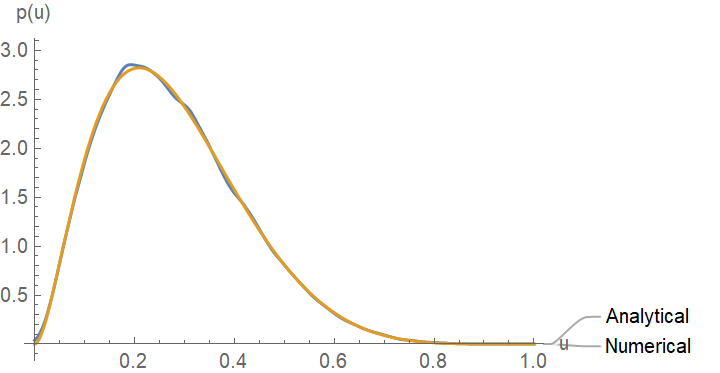
\includegraphics[width=0.95\textwidth,keepaspectratio]{014_001_Fig_Det_R.png}
\end{figure}

\subsubsection{Version History}
\begin{enumerate}
	\item \emph{First published: 12th Dec. 2021 on aravindhk-math.blogspot.com}
	\item \emph{Modified: 17th Dec. 2023 -- Style updates for \LaTeX}
\end{enumerate}
